\documentclass{article}

\usepackage{amsmath, graphicx}

\graphicspath{ {./images/} }

\title{Ch. 27 HW \#2 Solutions}
\author{Principles of Macroeconomics}
\date{today}

\begin{document}

\maketitle

\section*{Problems and Applications}

\begin{enumerate}

\item

	\begin{enumerate}
	
	\item Eastern European government  -- Lending to the U.S. government is probably less of a credit risk than lending to the Eastern European government because the economy is probably stronger and the government is probably more politically stable.
	
	\item 2050 -- A longer term leaves more time for the corporation to fall on hard times and potentially default, so longer term bonds pose a bigger credit risk.
	
	\item The software company -- The software company is less established and less well-known than Coca-Cola, so investors probably view it as a greater credit risk.
	
	\item Federal -- Interest earned on state bonds is exempt from the federal income tax, so state governments don't have to pay as much interest as the federal government.
	
	\end{enumerate}
	
\item Companies encourage workers to own stock in the firm because it gives them an ownership interest in the firm. That means they receive a portion of the firms’ future profits, so they’re more invested in their company’s success. That gives them a greater incentive to do high quality work. 

Employees might not want to hold stock in the company where they work because then they are highly dependent on the success of a single company. Both their wages and their savings depend on the success of that company. That’s riskier than diversifying their savings across a number of companies where they don’t work.


\setcounter{enumi}{7}
	
\item

	\begin{enumerate}
	
	\item If the government borrows more next year, then the budget deficit will increase. That will decrease public saving and therefore national saving. The supply of national saving will shift left, so the interest rate will rise.
	
	\begin{center}
	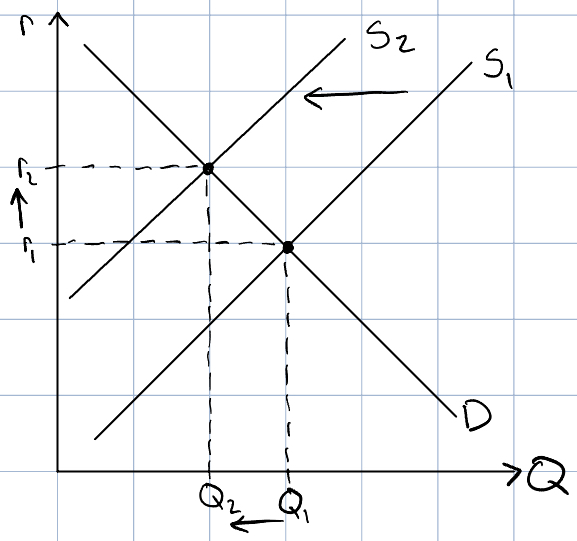
\includegraphics[width = 0.5\textwidth]{qfr6}
	\end{center}
	
	\item When the budget deficit increases by \$20 billion, public saving decreases by \$20 billion. As a result, the supply of loanable funds shifts left by \$20 billion, and the quantity of national saving and investment decreases. National saving and investment decrease by less than the \$20 billion shift in supply because the interest rate increases. When the interest rate increases, it incentivizes households to save more, so private saving increases and offsets some of the \$20 billion decrease in public saving. 
	
	\begin{center}
	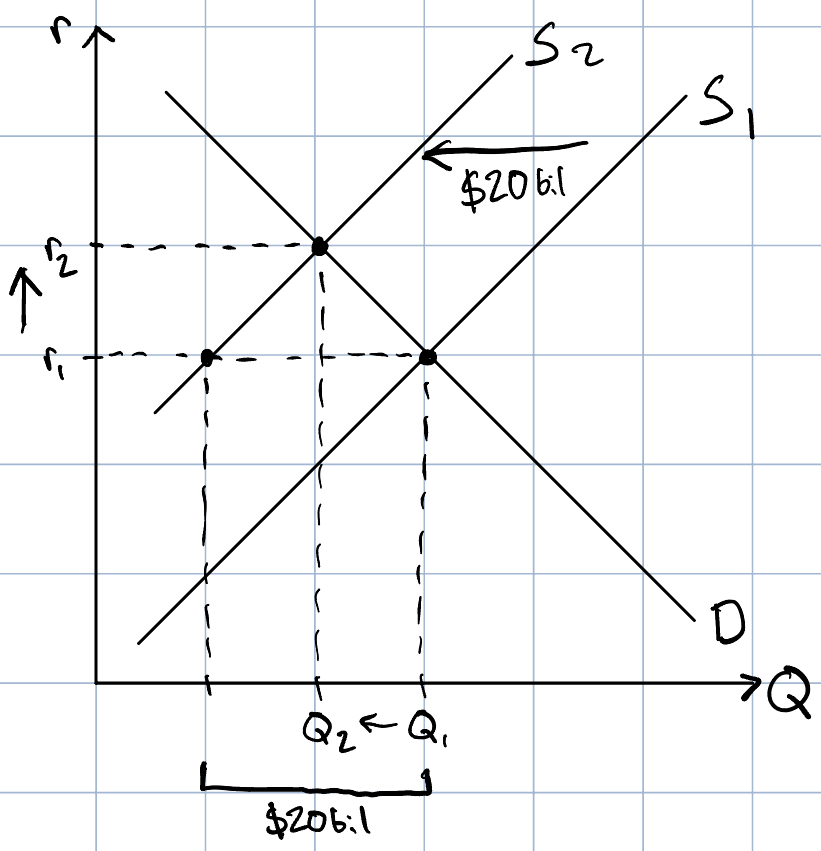
\includegraphics[width = 0.5\textwidth]{paa8b}
	\end{center}
	
	\item If the supply of loanable funds is more elastic, the decrease in public saving will be unaffected; the decrease in national saving and investment will be smaller, and the increase in private saving will be larger.
	
	\begin{center}
	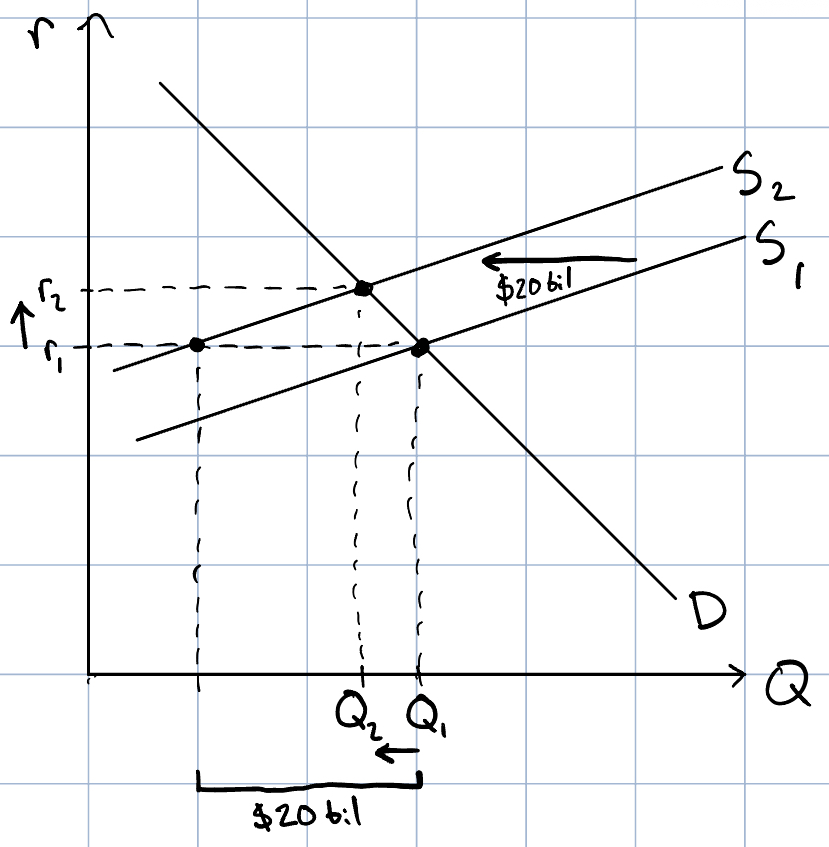
\includegraphics[width = 0.5\textwidth]{paa8c}
	\end{center}
	
	\item If the demand for loanable funds is more elastic, the decrease in public saving will be unaffected; the decrease in national saving and investment will be larger, and the increase in private saving will be smaller.
	
	\begin{center}
	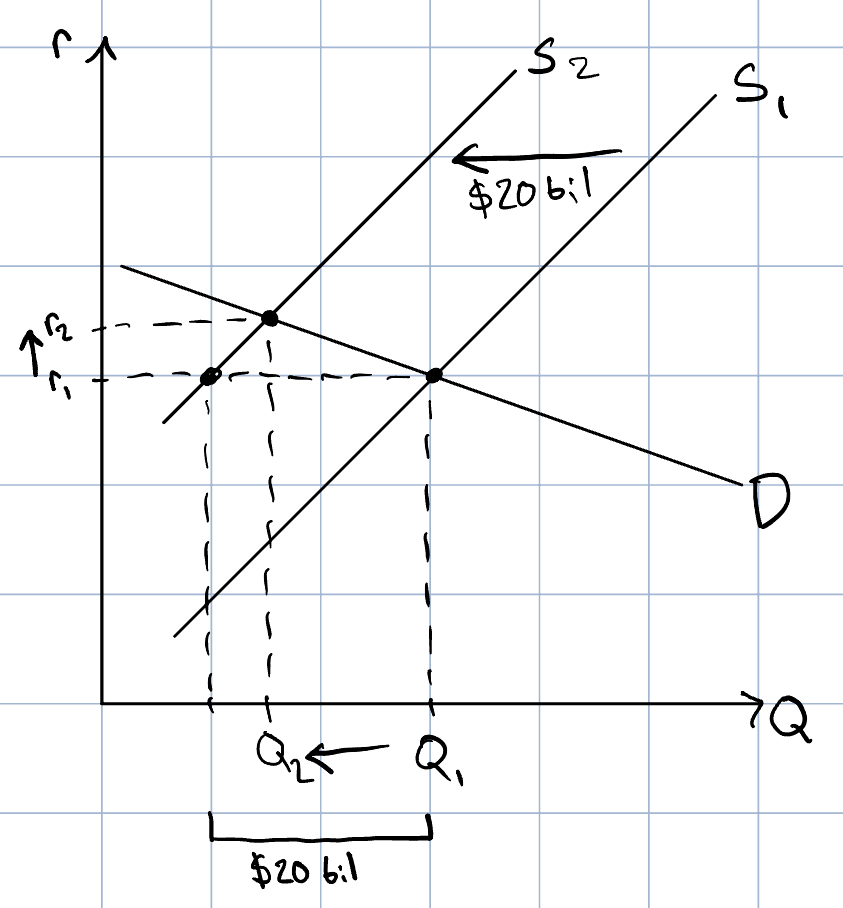
\includegraphics[width = 0.5\textwidth]{paa8d}
	\end{center}
	
	\item If households expected higher taxes in the future, they would save more today in order to pay those taxes in the future. Therefore, private saving would increase, and the supply of loanable funds would shift less than \$20 billion dollars to the left. That means. private saving would increase more, national saving would decrease less, investment would decrease less, and the interest rate would increase less than they did in parts (a) and (b). Public saving would still decrease by \$20 billion.
	
	\begin{center}
	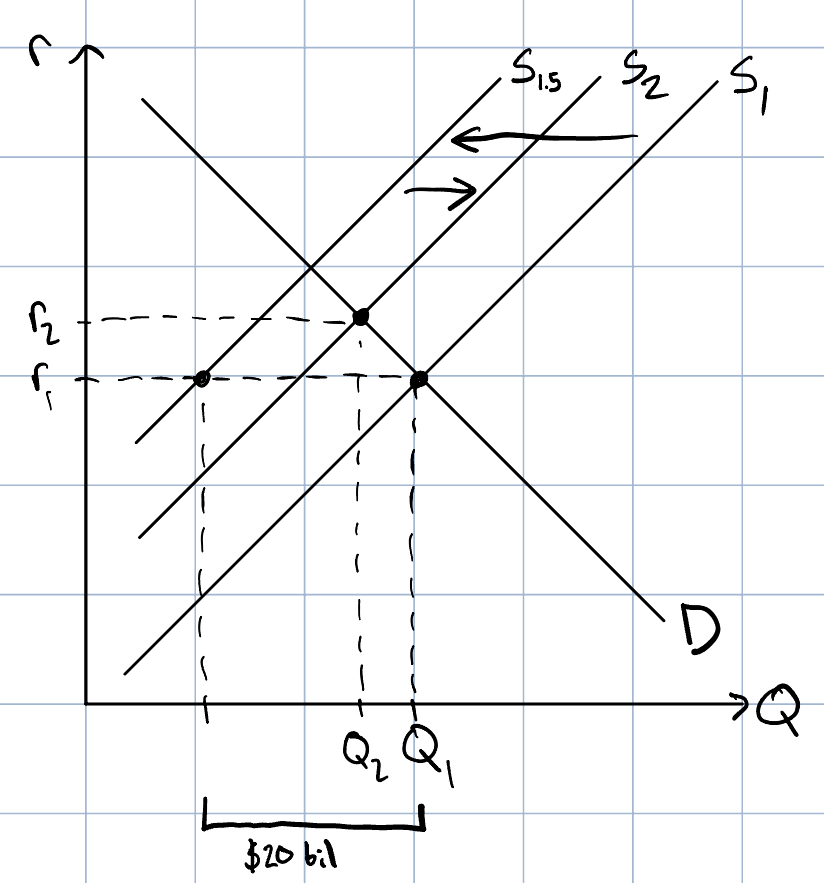
\includegraphics[width = 0.5\textwidth]{paa8e}
	\end{center}
	
	\end{enumerate}
	
\item

	\begin{enumerate}
	
	\item If government spending stays the same, a tax cut will increase the budget deficit. To cut taxes and reduce the deficit, the government would have to cut spending more than it cuts taxes.
	
	\item We would need to know how much private saving increases in response to a tax cut. A decrease in the government budget deficit increases public saving by the exact amount that the budget deficit decreases. It's less clear how responsive households are to tax cuts. Whichever policy increased saving more would increase investment more.
	
	\end{enumerate}

\end{enumerate}

\end{document}